
\begin{frame}[fragile]{Evaluationsmetrik}
  Zum Vergleich der generierten Rezensionen wird die ROUGE-Metrik verwendet.
  Die ROUGE-N Metrik misst die Anzahl der übereinstimmenden N-Grams zwischen dem generierten Text und den Referenztexten. 
  \begin{figure}[h!]
    \centering
\begin{tikzpicture}[
    box/.style={draw,rectangle,minimum size=1.3cm,text width=1.3cm,align=left}]
    \matrix (conmat) [row sep=.1cm,column sep=.1cm] {
    \node (tpos) [box,
        label=left:Positive,
        label=above:Positive,
        ] {True \\ positive};
    &
    \node (fneg) [box,
        label=above:Negative] {False \\ negative};
    \\
    \node (fpos) [box,
        label=left:Negative] {False \\ positive};
    &
    \node (tneg) [box] {True \\ negative};
    \\
    };
    \node [left=.05cm of conmat,text width=1.5cm,align=right] {\textbf{Referenz}};
    \node [above=.05cm of conmat] {\textbf{Vorhersage}};
\end{tikzpicture}
\caption{Konfusionsmatrix zur Berechnung des ROUGE-N Scores}
\end{figure}
\end{frame}


\begin{frame}{Evaluationsmetrik}
  % Zur Berechnung des ROUGE-N Scores werden die einzelnen Textabschnitte in eine Menge aus N-Grams zerlegt.
  % Mittels der Konfusionsmatrix in Abbildung  lassen sich Precision (P) und Recall (R) definieren:
      \textbf{Precision}: 
      Der Precision Wert ergibt sich aus dem Verhältnis der korrekt vorhergesagten N-Grams und der Anzahl der insgesamt vorhergesagten N-Grams.
      \begin{align*}
      \text{P} = \frac{\text{TP}}{\text{TP}+\text{FP}}
      \end{align*}
  
      \textbf{Recall}:
      Recall ist als Verhältnis zwischen den korrekt vorhergesagten N-Grams und den N-Grams aus der Referenz definiert.
      \begin{align*}
      \text{R} = \frac{\text{TP}}{\text{TP}+\text{FN}}
      \end{align*}
  
      \textbf{F1}:
      Das F1-Maß beschreibt das harmonische Mittel zwischen Precision und Recall.
      \begin{align*}
      \text{F}_\text{1} = \frac{2\text{PR}}{\text{P}+\text{R}}
      \end{align*}
\end{frame}

\begin{frame}{Ergebnisse}
  \begin{table}[!h]
  
    \centering
    \scalebox{0.8}{
    \begin{tabular}{@{}lcccc|cccc@{}}
    \toprule
             Test-Dataset                  & \multicolumn{4}{c}{Amazon} & \multicolumn{4}{c}{Yelp} \\ 
    \textbf{Method} & \textbf{R1} & \textbf{R2} & \textbf{RL} & \textbf{MV} & \textbf{R1} & \textbf{R2} & \textbf{RL} & \textbf{MV}\\ \midrule

    \rowcolor{gray!15} \textit{COOP + Attribute Model}        &         &         &        &        &        &   & &     \\
    \rowcolor{gray!15} $\quad$ Optimus            &   35.68   & \textbf{7.55}  &  20.68 & \textbf{56.73} &  33.85   &  6.98  & 18.82  &  56.47  \\ 
    \rowcolor{gray!15} $\quad$ \textsc{BiMeanVae}  &   \textbf{37.94}  &   7.20    &  \textbf{21.75} & \underline{56.69} &   \underline{34.97}  & \underline{7.06}     & \underline{19.86}  &  \textbf{56.90}  \\ \midrule

    \textit{COOP}              &         &         &        &        &        & &   &    \\ %PAPER
    $\quad$ Optimus   $^{\star}$          & 35.32 &6.22 &19.84  & 56.41&  33.68& 7.00 &18.95 & 56.41\\ 
    $\quad$ \textsc{BiMeanVae}  $^{\star}$   & \underline{36.57} &\underline{7.23} &\underline{21.24} & 56.49 & \textbf{35.37} & \textbf{7.35} &\textbf{19.94} & \underline{56.78} \\ \midrule
    
    \textit{SimpleAvg}                   &       &      &       &       &       &      &       & \\
    $\quad$ Optimus  $^{\star}$          & 33.54 & 6.18 & 19.34 & 56.49 & 31.23 & 6.48 & 18.27 & 56.15\\
    $\quad$ \textsc{BiMeanVae}$^{\star}$ & 33.60 & 6.64 & 20.87 & 55.85 & 32.87 & 6.93 & 19.89 & 56.36\\
    $\quad$ CopyCat  $^{\star}$          & 31.97 & 5.81 & 20.16 & -     & 29.47 & 5.26 & 18.09 & -\\ 
    $\quad$ MeanSum  $^{\star}$          & 29.20 & 4.70 & 18.15 & -     & 28.46 & 3.66 & 15.57 & -\\ \midrule
    \textit{Extractive}                  &       &      &       &       &       &      &       &      \\
    $\quad$ LexRank  $^{\star}$          & 28.74 & 5.47 & 16.75 & -     & 25.01 & 3.62 & 14.67 & -\\ \bottomrule
    \end{tabular}
    }
\end{table}
\end{frame}

\begin{frame}{Ergebnisse}

  \begin{itemize}
    \item Extraktive Methode LexRank unterliegt den abstraktiven Methoden in allen Metriken
    \item Abstraktive Methoden in SimpleAvg Gruppe: COOP Kombinationsmethode erzielt die höchste Performance
    \item COOP vs COOP + Attributmodell: 
    \begin{itemize}
      \item Attributmodell schafft es, die decodierten Textsequenzen in die gewünschte Richtung zu lenken und eine Leistungssteigerung zu erzielen
      \item Insbesondere spezifische Begriffe, die signifikant und damit ausschlaggebend für die erzeugten Rezensionen sind, allerdings in einer normalen Sprachverteilung eine geringe Gewichtung erhalten würden, werden durch das Bag of Words Attributmodell stark hervorgehoben
      \item Amazon-Datensatz: Outperformance des Attributmodells
      \item Yelp-Datensatz: \begin{itemize} \item Bessere Performance des Optimus Attributmodells
      \item möglicherweise keine Verbesserung aufgrund mangelnder Vergleichsrezensionen \end{itemize}
    \end{itemize}
  \end{itemize}
\end{frame}



\begin{frame}{Rezensionsauswahl durch Orakel}
  \begin{table}[!h]
  
    \centering
    \scalebox{0.8}{
      \begin{tabular}{@{}lcccc|cccc@{}}
        \toprule
                 Test-Dataset                  & \multicolumn{4}{c}{Amazon} & \multicolumn{4}{c}{Yelp} \\ 
        \textbf{Method} & \textbf{R1} & \textbf{R2} & \textbf{RL} & \textbf{MV} & \textbf{R1} & \textbf{R2} & \textbf{RL} & \textbf{MV}\\ \midrule
          
        \textit{COOP + Attribute Model}        &         &         &        &        &        &   & &     \\
        $\quad$ Optimus                         & 40.75 & \underline{8.82} & 21.54 & 56.88 & \underline{43.81} & \underline{11.08} & 22.43 & 57.34 \\ 
        $\quad$ \textsc{BiMeanVae}              & \textbf{42.15} & 8.67 & \textbf{23.52} & \textbf{57.18} & \textbf{45.13} & \textbf{11.23} & \textbf{24.77} & \textbf{57.82} \\ \midrule
        
        \textit{COOP}                           &       &      &       &       &       &       &       &        \\ %PAPER
        $\quad$ Optimus                          & 39.84 & 7.88 & 21.40 & \underline{57.02} & 42.05 & 10.03 & 22.24 & 57.32\\ 
        $\quad$ \textsc{BiMeanVae}               & \underline{40.80} & \textbf{8.99} & \underline{23.48} & 56.83 & 42.72 & 10.21 & \underline{24.00} & \underline{57.44} \\ \bottomrule
        \end{tabular}
    }
    % \caption{ROUGE und Moverscore Ergebnisse auf den Test-Benchmarkdatensätzen der unterschiedlichen Modelle mit Auswahl der generierten Rezensionen durch ein Orakel. Die besten Ergebnisse sind \textbf{fett} markiert und die zweitbesten Ergebnisse \underline{unterstrichen}.}
   
\end{table}
\begin{itemize}
\item Rezensionen wurden durch Orakel ausgewählt, um Rankingfunktionseinfluss zu vernachlässigen
\item Outperformance des COOP+Attributmodell in allen Bereichen
\end{itemize}
\end{frame}


\setlength{\fboxsep}{0.3em}


\begin{frame}{Beispielrezension Amazon}

  \begin{Rezension}[!h]
    \centering
    \scriptsize
    %\small
    \framebox{
      % 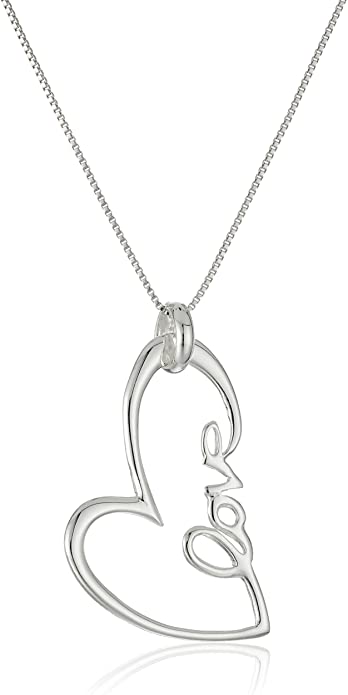
\includegraphics[width=1.3cm]{bilder/necklace.jpg}
        \parbox{\columnwidth-4\fboxsep}{
             \textbf{Produkt:} Sterling Silver \glqq{}Love\grqq{} Open Heart Pendant Necklace, 18\grqq{} \\ \\
        \textbf{\textsc{BiMeanVAE} COOP+Attribute-Model:} \ccolorbox[BackgroundColor]{ \textcolor{HighlightColor}{\strut This necklace}} \ccolorbox[BackgroundColor]{ \textcolor{HighlightColor}{\strut is a}} \ccolorbox[BackgroundColor]{ \textcolor{HighlightColor}{\strut great quality}} \textcolor{HighlightColor}{and} \textcolor{HighlightColor}{so} \textcolor{HighlightColor}{far} \textcolor{HighlightColor}{it}\textcolor{HighlightColor}{'s} \textcolor{HighlightColor}{the} perfect \textcolor{HighlightColor}{size}\ccolorbox[BackgroundColor]{\textcolor{HighlightColor}{\strut . It}} \ccolorbox[BackgroundColor]{ \textcolor{HighlightColor}{\strut is a}} \textcolor{HighlightColor}{very} \textcolor{HighlightColor}{nice} \textcolor{HighlightColor}{looking} \textcolor{HighlightColor}{necklace}\textcolor{HighlightColor}{,} \ccolorbox[BackgroundColor]{ \textcolor{HighlightColor}{\strut and the}} color \underline{\ccolorbox[BackgroundColor]{ \textcolor{HighlightColor}{\strut is beautiful}}\ccolorbox[BackgroundColor]{ \textcolor{HighlightColor}{\strut. The}} \ccolorbox[BackgroundColor]{ \textcolor{HighlightColor}{\strut chain is}} \textcolor{HighlightColor}{a}} perfect gift \ccolorbox[BackgroundColor]{ \textcolor{HighlightColor}{\strut for the}} \textcolor{HighlightColor}{price} \textcolor{HighlightColor}{of} \textcolor{HighlightColor}{the} necklace. I love \textcolor{HighlightColor}{it}\textcolor{HighlightColor}{!} \\ 
        \textbf{Scores:} R-1: 48.63, R-2: 16.78, R-L: 28.08, MV: 60.05\\ \\
        %\textbf{\textsc{BiMeanVAE} COOP:} \textcolor{HighlightColor}{This} \ccolorbox[BackgroundColor]{ \textcolor{HighlightColor}{\strut is a}} \textcolor{HighlightColor}{great} product \underline{\ccolorbox[BackgroundColor]{ \textcolor{HighlightColor}{\strut for the}} \ccolorbox[BackgroundColor]{ \textcolor{HighlightColor}{\strut price .}}} \textcolor{HighlightColor}{It} \ccolorbox[BackgroundColor]{ \textcolor{HighlightColor}{\strut is a}} \textcolor{HighlightColor}{very} \textcolor{HighlightColor}{good} \textcolor{HighlightColor}{quality} \textcolor{HighlightColor}{,} \ccolorbox[BackgroundColor]{ \textcolor{HighlightColor}{\strut and the}} \textcolor{HighlightColor}{price} was right \ccolorbox[BackgroundColor]{ \textcolor{HighlightColor}{\strut . The}} only thing \textcolor{HighlightColor}{is} that \ccolorbox[BackgroundColor]{ \textcolor{HighlightColor}{\strut it is}} \textcolor{HighlightColor}{a} little small \ccolorbox[BackgroundColor]{ \textcolor{HighlightColor}{\strut , but}} \textcolor{HighlightColor}{it} \textcolor{HighlightColor}{'s} not too big \ccolorbox[BackgroundColor]{ \textcolor{HighlightColor}{\strut . It}} \textcolor{HighlightColor}{'s} \ccolorbox[BackgroundColor]{ \textcolor{HighlightColor}{\strut a great}} buy \ccolorbox[BackgroundColor]{ \textcolor{HighlightColor}{\strut for the}} \ccolorbox[BackgroundColor]{ \textcolor{HighlightColor}{\strut price .}}  \\ 
        %\textbf{Scores:} R-1: 36.61, R-2: 8.30, R-L: 26.44, MV: 55.57 \\ \\
        \textbf{\textsc{BiMeanVAE} COOP:} \textcolor{HighlightColor}{It} was \textcolor{HighlightColor}{a} perfect gift \ccolorbox[BackgroundColor]{ \textcolor{HighlightColor}{for a}} friend \textcolor{HighlightColor}{of} her birthday\textcolor{HighlightColor}{.} She loves \textcolor{HighlightColor}{it}\textcolor{HighlightColor}{,} \textcolor{HighlightColor}{the} \textcolor{HighlightColor}{look} \textcolor{HighlightColor}{is} \textcolor{HighlightColor}{great}\textcolor{HighlightColor}{,} \ccolorbox[BackgroundColor]{ \textcolor{HighlightColor}{and the}} \textcolor{HighlightColor}{price} was \textcolor{HighlightColor}{great}\ccolorbox[BackgroundColor]{\textcolor{HighlightColor}{. It}} was easy \textcolor{HighlightColor}{to} set up\textcolor{HighlightColor}{,} \textcolor{HighlightColor}{and} she loves it. I \underline{\ccolorbox[BackgroundColor]{ \textcolor{HighlightColor}{would recommend}} \textcolor{HighlightColor}{this}} product \ccolorbox[BackgroundColor]{ \textcolor{HighlightColor}{to anyone}}\textcolor{HighlightColor}{.}   \\ 
        \textbf{Scores:} R-1: 33.56, R-2: 5.71, R-L: 20.27, MV: 56.00 \\ \\
    

        \textbf{Optimus COOP+Attribute-Model:} \textcolor{HighlightColor}{This} \ccolorbox[BackgroundColor]{ \textcolor{HighlightColor}{\strut is a}} \textcolor{HighlightColor}{great} gift \underline{\ccolorbox[BackgroundColor]{ \textcolor{HighlightColor}{\strut for the}} \ccolorbox[BackgroundColor]{ \textcolor{HighlightColor}{\strut price.}}} She loves \textcolor{HighlightColor}{it}\textcolor{HighlightColor}{,} \textcolor{HighlightColor}{so} much better than \textcolor{HighlightColor}{the} \textcolor{HighlightColor}{necklace} \textcolor{HighlightColor}{and} \textcolor{HighlightColor}{it} looks \ccolorbox[BackgroundColor]{ \textcolor{HighlightColor}{\strut beautiful.}} You \textcolor{HighlightColor}{can't} \textcolor{HighlightColor}{get} \textcolor{HighlightColor}{a} gift on \ccolorbox[BackgroundColor]{ \textcolor{HighlightColor}{\strut the chain}} \ccolorbox[BackgroundColor]{ \textcolor{HighlightColor}{\strut, but}} \ccolorbox[BackgroundColor]{ \textcolor{HighlightColor}{\strut it is}} not worth \textcolor{HighlightColor}{the} money\textcolor{HighlightColor}{!} \textcolor{HighlightColor}{It} looks \textcolor{HighlightColor}{great}\textcolor{HighlightColor}{!}         \\ 
        \textbf{Scores:} R-1: 42.65, R-2: 9.28, R-L: 26.57, MV: 58.31\\ \\
        % \textbf{Optimus COOP:}  \ So \textcolor{HighlightColor}{far} \textcolor{HighlightColor}{the} \underline{\ccolorbox[BackgroundColor]{ \textcolor{HighlightColor}{\strut necklace is}} \textcolor{HighlightColor}{beautiful}} \textcolor{HighlightColor}{,} \ccolorbox[BackgroundColor]{ \textcolor{HighlightColor}{\strut and the}} perfect gift \textcolor{HighlightColor}{for} someone who \ccolorbox[BackgroundColor]{ \textcolor{HighlightColor}{\strut is a}} \ccolorbox[BackgroundColor]{ \textcolor{HighlightColor}{\strut beautiful piece}} \ccolorbox[BackgroundColor]{ \textcolor{HighlightColor}{\strut . It}} looks \textcolor{HighlightColor}{great} on \textcolor{HighlightColor}{the} picture \ccolorbox[BackgroundColor]{ \textcolor{HighlightColor}{\strut , but}} \textcolor{HighlightColor}{it} does not \textcolor{HighlightColor}{look} like \textcolor{HighlightColor}{a} gift \textcolor{HighlightColor}{.} Im \textcolor{HighlightColor}{very} happy with \textcolor{HighlightColor}{this} \textcolor{HighlightColor}{necklace} \textcolor{HighlightColor}{and} \ccolorbox[BackgroundColor]{ \textcolor{HighlightColor}{\strut it is}} not worth \textcolor{HighlightColor}{the} money \textcolor{HighlightColor}{!}  \\ 
        % \textbf{Scores:} R-1: 40.26, R-2: 13.01, R-L: 23.48, MV: 58.06 }
        \textbf{Optimus COOP:}  Its \ccolorbox[BackgroundColor]{ \textcolor{HighlightColor}{a beautiful}} \textcolor{HighlightColor}{necklace}\textcolor{HighlightColor}{,} \textcolor{HighlightColor}{and} \textcolor{HighlightColor}{it} looks \textcolor{HighlightColor}{great} \underline{\ccolorbox[BackgroundColor]{ \textcolor{HighlightColor}{for the}} \ccolorbox[BackgroundColor]{ \textcolor{HighlightColor}{price.}}} She said \textcolor{HighlightColor}{it} was \textcolor{HighlightColor}{a} gift \textcolor{HighlightColor}{for} her birthday present\ccolorbox[BackgroundColor]{\textcolor{HighlightColor}{, but}} \ccolorbox[BackgroundColor]{ \textcolor{HighlightColor}{it is}} \textcolor{HighlightColor}{very} \textcolor{HighlightColor}{thin} \textcolor{HighlightColor}{and} not worth \textcolor{HighlightColor}{the} money\textcolor{HighlightColor}{.} If \textcolor{HighlightColor}{you} want \textcolor{HighlightColor}{to} go wrong with \textcolor{HighlightColor}{this} \textcolor{HighlightColor}{necklace}\textcolor{HighlightColor}{!}  \\ 
        \textbf{Scores:} R-1: 37.76, R-2: 8.57, R-L: 21.67, MV: 57.69 }
    
        }
    %\caption{Vergleich der generierten Rezensionen zwischen dem COOP und COOP + Attributionsmodell zu Produkt B0040EIHQQ des Amazon Datensatzes}

\end{Rezension}
\end{frame}

\begin{frame}{Beispielrezension Amazon}
  \begin{Rezension}[!h]
    \centering
    \scriptsize
    %\small 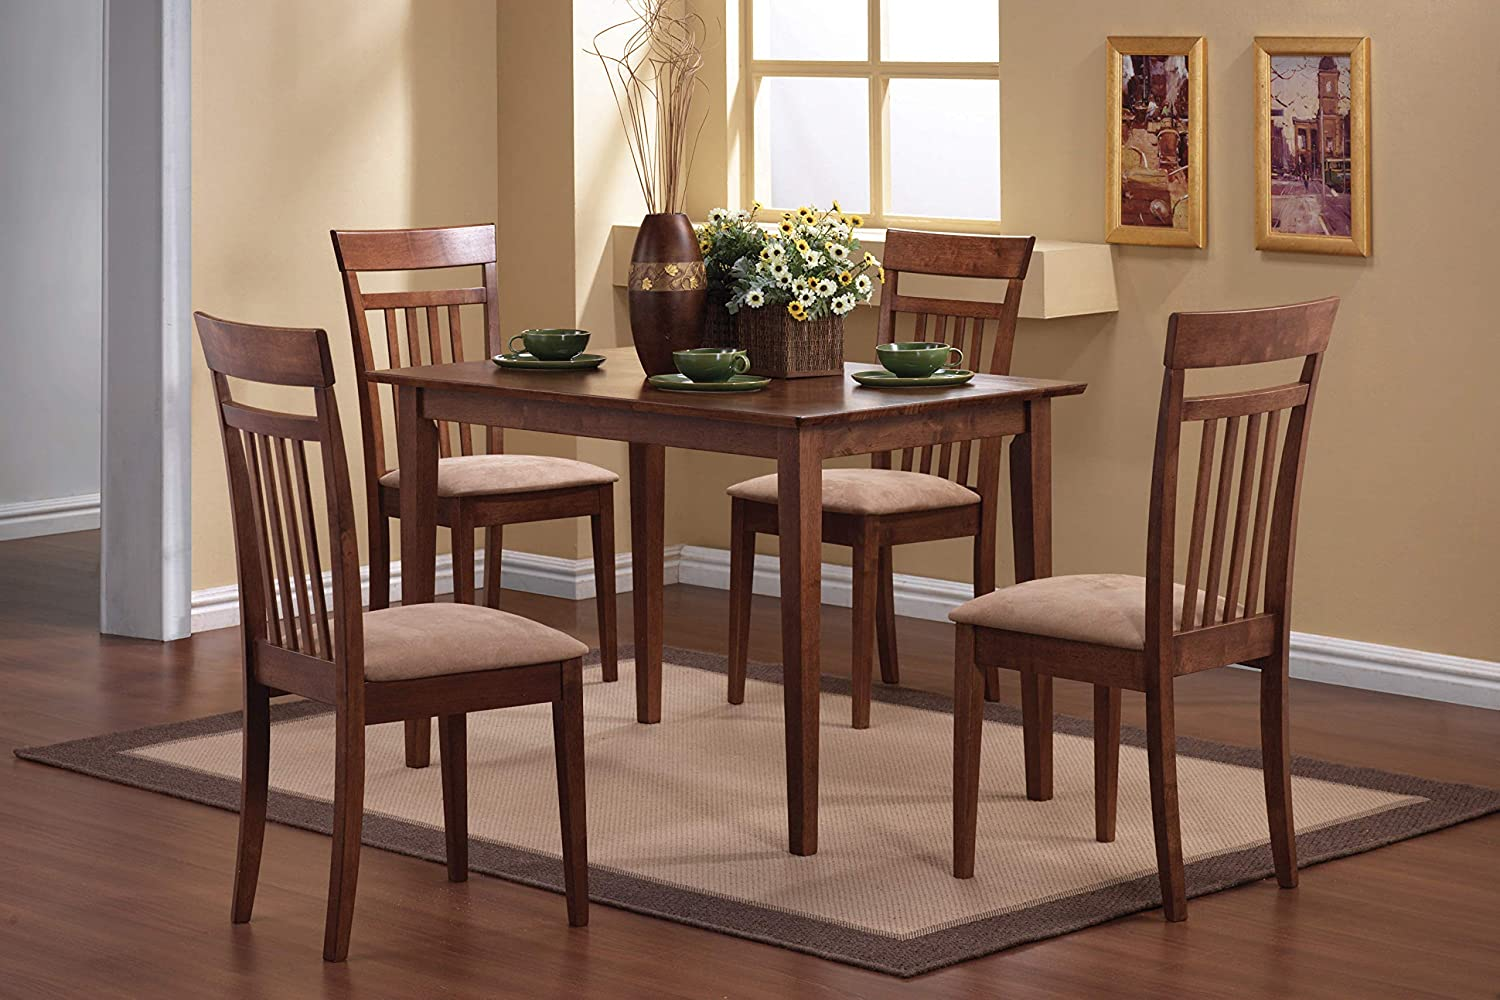
\includegraphics[width=1.5cm]{bilder/table.jpg}
    \framebox{
        \parbox{\columnwidth-4\fboxsep}{
             \textbf{Produkt:} Coaster CO-150430 5 Pc Dining Set, Chestnut \\ \\
        \textbf{\textsc{BiMeanVAE} COOP+Attribute-Model:} \textcolor{HighlightColor}{The} table \ccolorbox[BackgroundColor]{ \textcolor{HighlightColor}{is very}} \textcolor{HighlightColor}{nice} \textcolor{HighlightColor}{and} \textcolor{HighlightColor}{sturdy}\ccolorbox[BackgroundColor]{\textcolor{HighlightColor}{. It}} \textcolor{HighlightColor}{was} \ccolorbox[BackgroundColor]{ \textcolor{HighlightColor}{easy to}} \ccolorbox[BackgroundColor]{ \textcolor{HighlightColor}{put together}} \textcolor{HighlightColor}{and} \textcolor{HighlightColor}{the} \textcolor{HighlightColor}{color} \textcolor{HighlightColor}{is} perfect\ccolorbox[BackgroundColor]{\textcolor{HighlightColor}{. The}} \textcolor{HighlightColor}{chairs} \textcolor{HighlightColor}{are} \textcolor{HighlightColor}{a} bit \textcolor{HighlightColor}{small} \textcolor{HighlightColor}{for} \textcolor{HighlightColor}{the} price\ccolorbox[BackgroundColor]{\textcolor{HighlightColor}{, but}} \textcolor{HighlightColor}{it}'s \textcolor{HighlightColor}{not} \textcolor{HighlightColor}{a} big \textcolor{HighlightColor}{deal}\ccolorbox[BackgroundColor]{\textcolor{HighlightColor}{. It}} \textcolor{HighlightColor}{was} \underline{\ccolorbox[BackgroundColor]{ \textcolor{HighlightColor}{very easy}} \ccolorbox[BackgroundColor]{ \textcolor{HighlightColor}{to assemble}}\textcolor{HighlightColor}{.}}        \\ 
        \textbf{Scores:} R-1: 42.75, R-2: 7.03, R-L: 23.66, MV: 54.49\\ \\
        \textbf{\textsc{BiMeanVAE} COOP:} \textcolor{HighlightColor}{The} table \ccolorbox[BackgroundColor]{ \textcolor{HighlightColor}{is very}} \textcolor{HighlightColor}{nice} \textcolor{HighlightColor}{and} \textcolor{HighlightColor}{sturdy}\ccolorbox[BackgroundColor]{\textcolor{HighlightColor}{. The}} \textcolor{HighlightColor}{chairs} \textcolor{HighlightColor}{are} \underline{\ccolorbox[BackgroundColor]{ \textcolor{HighlightColor}{easy to}} \ccolorbox[BackgroundColor]{ \textcolor{HighlightColor}{put together}}} \textcolor{HighlightColor}{and} \textcolor{HighlightColor}{the} \textcolor{HighlightColor}{color} \textcolor{HighlightColor}{is} \textcolor{HighlightColor}{great}\ccolorbox[BackgroundColor]{\textcolor{HighlightColor}{. It}} \textcolor{HighlightColor}{was} \ccolorbox[BackgroundColor]{ \textcolor{HighlightColor}{easy to}} \textcolor{HighlightColor}{assemble}\textcolor{HighlightColor}{,} \textcolor{HighlightColor}{and} \textcolor{HighlightColor}{the} price \textcolor{HighlightColor}{was} right\ccolorbox[BackgroundColor]{\textcolor{HighlightColor}{. The}} \textcolor{HighlightColor}{size} \textcolor{HighlightColor}{is} perfect \ccolorbox[BackgroundColor]{ \textcolor{HighlightColor}{for a}} \textcolor{HighlightColor}{small} kitchen\textcolor{HighlightColor}{,} \textcolor{HighlightColor}{so} \textcolor{HighlightColor}{it}'s \textcolor{HighlightColor}{not} \textcolor{HighlightColor}{a} big \textcolor{HighlightColor}{deal}\textcolor{HighlightColor}{.}         \\ 
        \textbf{Scores:} R-1: 41.60, R-2: 9.70, R-L: 24.81, MV: 54.53 \\ \\

        \textbf{Optimus COOP+Attribute-Model:} Just received this table \textcolor{HighlightColor}{top} \textcolor{HighlightColor}{and} \textcolor{HighlightColor}{sturdy}\ccolorbox[BackgroundColor]{\textcolor{HighlightColor}{. The}} table \textcolor{HighlightColor}{is} perfect \textcolor{HighlightColor}{for} \textcolor{HighlightColor}{the} price\textcolor{HighlightColor}{,} \textcolor{HighlightColor}{so} \textcolor{HighlightColor}{it} \textcolor{HighlightColor}{was} \underline{\ccolorbox[BackgroundColor]{ \textcolor{HighlightColor}{easy to}}\ccolorbox[BackgroundColor]{\textcolor{HighlightColor}{assemble.}}} One \ccolorbox[BackgroundColor]{ \textcolor{HighlightColor}{of the}} \textcolor{HighlightColor}{chairs} \textcolor{HighlightColor}{are} \textcolor{HighlightColor}{not} \ccolorbox[BackgroundColor]{ \textcolor{HighlightColor}{sturdy,}} \textcolor{HighlightColor}{sturdy} \textcolor{HighlightColor}{and} \textcolor{HighlightColor}{the} table \textcolor{HighlightColor}{was} \textcolor{HighlightColor}{not} worth \textcolor{HighlightColor}{the} money\textcolor{HighlightColor}{.} Other than \ccolorbox[BackgroundColor]{ \textcolor{HighlightColor}{that it}} \textcolor{HighlightColor}{is} \textcolor{HighlightColor}{a} \textcolor{HighlightColor}{great} \ccolorbox[BackgroundColor]{ \textcolor{HighlightColor}{purchase.}}         \\ 
        \textbf{Scores:} R-1: 32.85, R-2: 5.22, R-L: 20.44, MV: 53.52 \\ \\
        \textbf{Optimus COOP:} Just received this table \textcolor{HighlightColor}{and} \textcolor{HighlightColor}{sturdy}\ccolorbox[BackgroundColor]{\textcolor{HighlightColor}{. The}} table \textcolor{HighlightColor}{is} perfect \textcolor{HighlightColor}{for} \textcolor{HighlightColor}{the} price\textcolor{HighlightColor}{,} \ccolorbox[BackgroundColor]{ \textcolor{HighlightColor}{and it}} \textcolor{HighlightColor}{was} \underline{\ccolorbox[BackgroundColor]{ \textcolor{HighlightColor}{easy to}} \ccolorbox[BackgroundColor]{ \textcolor{HighlightColor}{assemble.}}} One \ccolorbox[BackgroundColor]{ \textcolor{HighlightColor}{of the}} \textcolor{HighlightColor}{chairs} \textcolor{HighlightColor}{are} \textcolor{HighlightColor}{not} perfect\ccolorbox[BackgroundColor]{\textcolor{HighlightColor}{. It}} \textcolor{HighlightColor}{is} \textcolor{HighlightColor}{sturdy} \textcolor{HighlightColor}{and} \textcolor{HighlightColor}{not} worth \textcolor{HighlightColor}{the} money\textcolor{HighlightColor}{.}         \\ 
        \textbf{Scores:} R-1: 30.32, R-2: 6.72, R-L: 19.67, MV: 53.49 }
    }
    % \caption{Vergleich der generierten Rezensionen zwischen dem COOP und COOP+Attributmodell zu Produkt B001EQJ5AU des Amazon Datensatzes}
    % \label{reviewAmz2}
\end{Rezension}
\end{frame}

\begin{frame}{Beispielrezension Yelp}
  \begin{Rezension}[!h] %60
    \centering
    \scriptsize
    % \small
    \framebox{
        \parbox{\columnwidth-4\fboxsep}{
        \textbf{Restaurant:} Harbour 60 Steakhouse \\ 
        \textbf{Referenz:} This place has some amazing, tasty steaks!  They are breathtaking!  The menu also has seafood options that are just as delicious!  The only downside is that its pretty expensive, however you get top quality meat for what you pay for.  You won't even notice the price when your stomach is filled with the best seasoned meat you've ever had.
        \\ \\
        \textbf{\textsc{BiMeanVAE} COOP+Attribute-Model:} \underline{\ccolorbox[BackgroundColor]{ \textcolor{HighlightColor}{This place}}} \textcolor{HighlightColor}{is} a great \textcolor{HighlightColor}{place} to eat\textcolor{HighlightColor}{.} \textcolor{HighlightColor}{The} food \textcolor{HighlightColor}{is} very good and \textcolor{HighlightColor}{the} service \textcolor{HighlightColor}{is} excellent\textcolor{HighlightColor}{.} It's a little pricey but it's worth it \textcolor{HighlightColor}{for} \textcolor{HighlightColor}{the} \textcolor{HighlightColor}{quality} of \textcolor{HighlightColor}{the} food and \textcolor{HighlightColor}{the} service\textcolor{HighlightColor}{.} \textcolor{HighlightColor}{The} steak was cooked to perfection and \textcolor{HighlightColor}{the} lobster bisque was \textcolor{HighlightColor}{delicious}\textcolor{HighlightColor}{.} \textcolor{HighlightColor}{The} \textcolor{HighlightColor}{best} part of \textcolor{HighlightColor}{the} meal was \textcolor{HighlightColor}{the} wine\textcolor{HighlightColor}{.}         \\ 
        \textbf{Scores:} R-1: 21.85, R-2: 5.13, R-L: 15.13, MV: 56.57\\ 
        \textbf{\textsc{BiMeanVAE} COOP:} Excellent food and great service\textcolor{HighlightColor}{.} \textcolor{HighlightColor}{The} staff \textcolor{HighlightColor}{is} very friendly and \textcolor{HighlightColor}{the} food \textcolor{HighlightColor}{is} \textcolor{HighlightColor}{delicious}\textcolor{HighlightColor}{.} \textcolor{HighlightColor}{The} steak was cooked to perfection and \textcolor{HighlightColor}{the} service was a little slow but it was worth \textcolor{HighlightColor}{the} wait\textcolor{HighlightColor}{.} It's a great \underline{\textcolor{HighlightColor}{place}} to go \textcolor{HighlightColor}{for} a date night\textcolor{HighlightColor}{.}         \\ 
        \textbf{Scores:} R-1: 18.86, R-2: 1.92, R-L: 9.43, MV: 55.69 \\ 

        \textbf{Optimus COOP+Attribute-Model:} One of \underline{\ccolorbox[BackgroundColor]{ \textcolor{HighlightColor}{the best}}} steakhouse\textcolor{HighlightColor}{.} It's a great meal\textcolor{HighlightColor}{.} \textcolor{HighlightColor}{The} service was \textcolor{HighlightColor}{amazing} and \textcolor{HighlightColor}{the} food was \textcolor{HighlightColor}{delicious}\textcolor{HighlightColor}{.} If \textcolor{HighlightColor}{you}'re looking \textcolor{HighlightColor}{for} a long time to eat at \textcolor{HighlightColor}{the} strip\ccolorbox[BackgroundColor]{\textcolor{HighlightColor}{. You}} ca\textcolor{HighlightColor}{n't} wait \textcolor{HighlightColor}{for} dinner\textcolor{HighlightColor}{.} \textcolor{HighlightColor}{This} \textcolor{HighlightColor}{is} a little pricey \textcolor{HighlightColor}{for} \textcolor{HighlightColor}{the} steak and it was perfect\textcolor{HighlightColor}{.} Highly recommend this \textcolor{HighlightColor}{place} to anyone in town\textcolor{HighlightColor}{.}         \\ 
        \textbf{Scores:} R-1: 26.89, R-2: 3.42, R-L: 15.13, MV: 57.28 \\ 
        \textbf{Optimus COOP:} \textcolor{HighlightColor}{This} restaurant \textcolor{HighlightColor}{is} a great \textcolor{HighlightColor}{place} to die \ccolorbox[BackgroundColor]{ \textcolor{HighlightColor}{for.}} \textcolor{HighlightColor}{The} food \textcolor{HighlightColor}{is} \textcolor{HighlightColor}{amazing} and \textcolor{HighlightColor}{the} service \textcolor{HighlightColor}{is} fantastic\textcolor{HighlightColor}{.} It's a little pricey but \textcolor{HighlightColor}{the} food was \textcolor{HighlightColor}{delicious}\textcolor{HighlightColor}{.} Everything was perfect \textcolor{HighlightColor}{for} \textcolor{HighlightColor}{the} steak and \underline{\ccolorbox[BackgroundColor]{ \textcolor{HighlightColor}{delicious!}} \textcolor{HighlightColor}{The}} service was great\textcolor{HighlightColor}{,} \ccolorbox[BackgroundColor]{ \textcolor{HighlightColor}{the best}} part of \textcolor{HighlightColor}{the} restaurant in \textcolor{HighlightColor}{the} city\textcolor{HighlightColor}{.} If \textcolor{HighlightColor}{you} want to go back \textcolor{HighlightColor}{for} dinner\textcolor{HighlightColor}{,} it's not worth it\textcolor{HighlightColor}{.}         \\ 
        \textbf{Scores:} R-1: 24.39, R-2: 3.30, R-L: 16.26, MV: 57.52  

        }
    }
    % \caption{Vergleich der generierten Rezensionen zwischen dem COOP und COOP+Attributmodell zu Dienstleistung 4POPYEONJpkfhWOMx\_PyGg des Yelp Datensatzes} %4POPYEONJpkfhWOMx_PyGg
    % \label{reviewYelp1}
\end{Rezension}
\end{frame}

\begin{frame}{Beispielrezension Yelp}
  \begin{Rezension}[!h] %85
    \centering
    \scriptsize
    % \small
    \framebox{
        \parbox{\columnwidth-4\fboxsep}{
        \textbf{Restaurant:} Anna Marie's Italian Cuisine \\ 
        \textbf{Referenz:} Great place to go food authentic Italian food. Pizza is amazing, lots of topping choices  and they aren't stingy with them. Drinks and desert wont disappoint either. The atmosphere is pleasant, and provides a nice escape from the heat. Staff can be hit or miss but the place is clean and they have some good happy hour deals.
        \\ \\
        \textbf{\textsc{BiMeanVAE} COOP+Attribute-Model:} Had \textcolor{HighlightColor}{a} great experience here\ccolorbox[BackgroundColor]{\textcolor{HighlightColor}{. The}} \textcolor{HighlightColor}{food} was very \textcolor{HighlightColor}{good} \textcolor{HighlightColor}{and} \textcolor{HighlightColor}{the} service was excellent\textcolor{HighlightColor}{.} It's \ccolorbox[BackgroundColor]{ \textcolor{HighlightColor}{a nice}} \underline{\ccolorbox[BackgroundColor]{ \textcolor{HighlightColor}{place to}} \textcolor{HighlightColor}{go}} \textcolor{HighlightColor}{with} \textcolor{HighlightColor}{a} group \textcolor{HighlightColor}{of} friends \textcolor{HighlightColor}{and} family\textcolor{HighlightColor}{.} They \textcolor{HighlightColor}{have} \textcolor{HighlightColor}{a} great \ccolorbox[BackgroundColor]{ \textcolor{HighlightColor}{happy hour}} menu \textcolor{HighlightColor}{and} \textcolor{HighlightColor}{the} \textcolor{HighlightColor}{food} \textcolor{HighlightColor}{is} very \textcolor{HighlightColor}{good}\textcolor{HighlightColor}{.} If you \textcolor{HighlightColor}{are} in \textcolor{HighlightColor}{the} area\textcolor{HighlightColor}{,} this \textcolor{HighlightColor}{is} \textcolor{HighlightColor}{a} must try\textcolor{HighlightColor}{.}         \\ 
        \textbf{Scores:} R-1: 41.07, R-2: 9.09, R-L: 21.43, MV: 57.87\\ 
        \textbf{\textsc{BiMeanVAE} COOP:} Came here for \textcolor{HighlightColor}{the} first time \textcolor{HighlightColor}{and} it was \textcolor{HighlightColor}{a} great experience\ccolorbox[BackgroundColor]{\textcolor{HighlightColor}{. The}} \textcolor{HighlightColor}{food} was delicious \textcolor{HighlightColor}{and} \textcolor{HighlightColor}{the} staff was very friendly\underline{\ccolorbox[BackgroundColor]{\textcolor{HighlightColor}{. The}} \ccolorbox[BackgroundColor]{ \textcolor{HighlightColor}{atmosphere is}}} \textcolor{HighlightColor}{nice} \textcolor{HighlightColor}{and} \textcolor{HighlightColor}{the} service was \textcolor{HighlightColor}{good}\textcolor{HighlightColor}{.} It's \textcolor{HighlightColor}{a} great \ccolorbox[BackgroundColor]{ \textcolor{HighlightColor}{place to}} \textcolor{HighlightColor}{go} if you \textcolor{HighlightColor}{are} in \textcolor{HighlightColor}{the} area\textcolor{HighlightColor}{.}         \\ 
        \textbf{Scores:} R-1: 33.00, R-2: 9.90, R-L: 17.47, MV: 56.94 \\ 

        \textbf{Optimus COOP+Attribute-Model:} Came here for \textcolor{HighlightColor}{a} few weeks ago\textcolor{HighlightColor}{.} It was very friendly \textcolor{HighlightColor}{and} \textcolor{HighlightColor}{the} \textcolor{HighlightColor}{food} was delicious\textcolor{HighlightColor}{.} They \textcolor{HighlightColor}{have} \textcolor{HighlightColor}{a} great experience\underline{\ccolorbox[BackgroundColor]{\textcolor{HighlightColor}{. The}}} \textcolor{HighlightColor}{food} \textcolor{HighlightColor}{is} very \textcolor{HighlightColor}{nice} \textcolor{HighlightColor}{and} it was \textcolor{HighlightColor}{a} bit \textcolor{HighlightColor}{of} \textcolor{HighlightColor}{the} best pizza\textcolor{HighlightColor}{.} If you want \ccolorbox[BackgroundColor]{ \textcolor{HighlightColor}{to go}} back \textcolor{HighlightColor}{to} try \textcolor{HighlightColor}{the} menu\textcolor{HighlightColor}{.} Definitely will definitely \textcolor{HighlightColor}{be} back \textcolor{HighlightColor}{and} try this \textcolor{HighlightColor}{place}\textcolor{HighlightColor}{.}         \\ 
        \textbf{Scores:} R-1: 35.40, R-2: 3.60, R-L: 15.93, MV: 56.91 \\ 
        \textbf{Optimus COOP:} Absolutely love this \textcolor{HighlightColor}{place}! \textcolor{HighlightColor}{The} \textcolor{HighlightColor}{food} was very friendly \textcolor{HighlightColor}{and} \textcolor{HighlightColor}{the} service was excellent\ccolorbox[BackgroundColor]{\textcolor{HighlightColor}{. The}} staff \textcolor{HighlightColor}{is} very \textcolor{HighlightColor}{nice} \textcolor{HighlightColor}{and} attentive\textcolor{HighlightColor}{.} They \textcolor{HighlightColor}{have} \underline{\ccolorbox[BackgroundColor]{ \textcolor{HighlightColor}{a nice}}} \textcolor{HighlightColor}{atmosphere} \textcolor{HighlightColor}{and} made it out \textcolor{HighlightColor}{of} \textcolor{HighlightColor}{the} menu\textcolor{HighlightColor}{.} It's \textcolor{HighlightColor}{a} must try \textcolor{HighlightColor}{to} come back\textcolor{HighlightColor}{.} Definitely will definitely \textcolor{HighlightColor}{be} back!         \\ 
        \textbf{Scores:} R-1: 34.28, R-2: 3.88, R-L: 19.04, MV: 56.75  
        }
    }
    % \caption{Vergleich der generierten Rezensionen zwischen dem COOP und COOP+Attributmodell zu Dienstleistung 6jDD-Z8QcsKTdIDWwM8gog des Yelp Datensatzes}
    % \label{reviewYelp2}
\end{Rezension}
\end{frame}



